Programmer profesional menggunakan cara yang efektif dan seefisien mungkin dalam menyelesaikan suatu permasalahan. Menemukan cara yang efektif dan efisien salah satu caranya yaitu dengan meminimalisir kompleksitas dari algoritma yang digunakan.
Kompleksitas suatu algoritma terbagi menjadi 2, yaitu Time Complexity dan Space Complexity.

Time Complexity merupakan lama waktu yang diperlukan untuk menjalankan suatu algoritma. Sedangkan Space Complexity adalah ukuran ruang penyimpanan yang kita gunakan untuk menjalankan suatu algoritma. Dan disini saya hanya akan membahas tentang Time Complexity. Sebelum itu saya ingin teman-teman memahami terlebih dahulu apa itu algoritma. Sederhananya, algoritma adalah serangkaian proses yang dilakukan secara berurutan untuk menyelesaikan sebuah permasalahan. Algoritma bisa bermacam-macam tergantung kepada siapa yang membuat algoritma tersebut. Namun permasalahannya adalah menentukan algortima mana yang lebih efektif dan efisien untuk menyelesaikan permasalahan yang kita hadapi.

Contoh simpel dalam kehidupan kita sehari-hari, ketika kita ingin pergi ke suatu tempat tetapi ada banyak jalan yang bisa kita lalui untuk bisa sampai di tempat tujuan, namun permasalahannya adalah rute mana yang paling cepat yang bisa kita ambil untuk sampai di tempat tujuan.

Time Complexity Analysis adalah suatu cara sederhana untuk mengetahui berapa lama waktu yang dibutuhkan untuk menjalankan suatu algoritma dengan input tertentu (n). Biasanya lebih dikenal dengan sebutan Big-O Notation. Big O Notation digunakan untuk mengukur tingkat kompleksitas suatu algoritma. Big-O Notation adalah cara untuk mengkonversi keseluruhan langkah-langkah suatu algoritma kedalam bentuk Aljabar, yaitu dengan menghiraukan konstanta yang lebih kecil dan koefisien yang tidak berdampak besar terhadap keseluruhan kompleksitas permasalahan yang diselesaikan oleh algoritma tersebut. Mari kita liat contoh dibawah ini:

\begin{table}[]
\begin{tabular}{ll}
Regular               & Big O                                                                 \\
2                     & O(1) = it's just a constant number                                    \\
2n + 10               & O(n) = n has the largest effect                                       \\
5n\textasciicircum{}2 & O(n\textasciicircum{}2) = n\textasciicircum{}2 has the largest effect
\end{tabular}
\end{table}

Sederhananya, semua contoh yang ada diatas mengatakan bahwa “kita hanya akan melihat faktor yang memiliki dampak paling besar terhadap nilai yang dihasilkan oleh algoritma tersebut”.

Terdapat beberapa macam time complexity, diantaranya:
\begin{enumerate}
\item O(1) — Constant Time
Constant Time artinya banyaknya input yang diberikan kepada sebuah algoritma, tidak akan mempengaruhi waktu proses (runtime) dari algoritma tersebut. Suatu algoritma dengan T( n )  O(1) dikatakan memiliki kompleksitas waktu yang konstan.
\begin{lstlisting}
let myArray = [1, 5, 0, 6, 1, 9, 9, 2];
function getFirst(input){
   return input[0]; // selalu melakukan 1 langkah
}
let firstEl = getFirst(myArray);
\end{lstlisting}
Contoh diatas, terdapat sebuah fungsi untuk mengambil elemen pertama dari sebuah input array. Kita bisa melihat bahwa berapapun jumlah array yang diberikan kepada fungsi tersebut, dia akan selalu melakukan 1 hal, yaitu mengambil elemen pertama. Itu artinya jumlah input yang diberikan tidak mempengaruhi waktu proses (runtime) dari algoritma tersebut.
\begin{figure}[H]
    \centering
    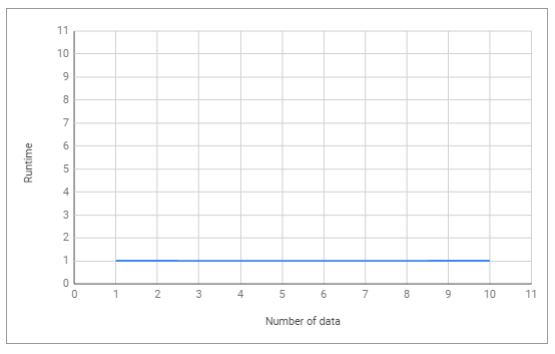
\includegraphics[scale=0.5]{figures/cons_time}
    \caption{\textit{Constant Time}}
    \label{cons}
\end{figure}

\item O(log n) — Logarithmic Time
Logarithmic Time artinya ketika kita memberikan input sebesar n terhadap sebuah fungsi, jumlah tahapan yang dilakukan oleh fungsi tersebut berkurang berdasarkan suatu faktor. Salah satu contohnya adalah algoritma Binary Search.
Binary Search adalah algoritma yang kita gunakan dalam mencari posisi nilai dari suatu array dengan cara ‘mengeliminasi’ setengah dari array input untuk mempercepat proses pencarian.
\begin{lstlisting}
let sortedArray = [11, 24, 30, 43, 51, 61, 73, 86];
function isExists(number, array){
    var midPoint = Math.floor( array.length /2 );
    if( array[midPoint] === num) return true;
    let isFirstHalf = false;
    if( array[midPoint] < num ) isFirstHalf = true;
  
    else if( array[midpoint] > num ) isFirstHalf = false;
    if (array.length == 1) return false;
    else { 
        // memanggil fungsi yang sama dengan mengeleminiasi setengah dari input array
        if (isFirstHalf) 
            return isExists(number, getFirstHalf(array));
        else 
            return isExists(number, getSecondHalf(array));
    }
}
isExists (24, sortedArray); // return true
isExists (27, sortedArray); // return false
\end{lstlisting}

\begin{figure}[H]
    \centering
    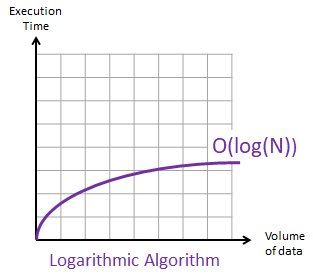
\includegraphics[scale=0.5]{figures/logarithmic}
    \caption{\textit{Logarithmic Time}}
    \label{logarithmic}
\end{figure}

\item O(n) — Linear Time
Linear Time adalah ketika runtime dari fungsi kita berbanding lurus dengan jumlah input yang diberikan.
\begin{lstlisting}
let myArray = [1, 5, 0, 6, 1, 9, 9, 2];
function getMax(input){
    var max = 0;
    for (var i=0; i<input.length; i++){
        if (max < input[i])
            max = input[i];
    }
    return max;
}
let maxNumber = getMax(myArray);
\end{lstlisting}
Kita bisa melihat bahwa semakin banyak jumlah input yang diberikan, maka waktu proses/runtime dari fungsi tersebut akan semakin besar.
\begin{figure}[H]
    \centering
    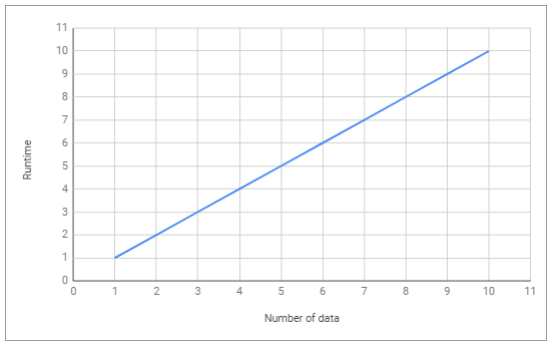
\includegraphics[scale=0.5]{figures/linear_time}
    \caption{\textit{Linear Time}}
    \label{linear}
\end{figure}

\item O(n²) — Quadratic Time
Quadratic Time adalah ketika runtime dari fungsi kita adalah sebesar n\^2, dimana n adalah jumlah input dari fungsi tersebut. Hal tersebut bisa terjadi karena kita menjalankan fungsi linear didalam fungsi linear (n*n).
\begin{lstlisting}
let myArray = [1, 5, 0, 6, 1, 9, 9, 2];
function sort(input){
    var sortedArray = [];
    for (var i=0; i<input.length; i++){ // O(n)
        let min = input[i];
        for (var j=i+1; i<input.length; i++){ // O(n)
            if (input[i] < input[j])
                min = input[j];
        }
        sortedArray.push(min);
    }
    return sortedArray;
}
let sortedArray = sort(myArray);
\end{lstlisting}
\begin{figure}[H]
    \centering
    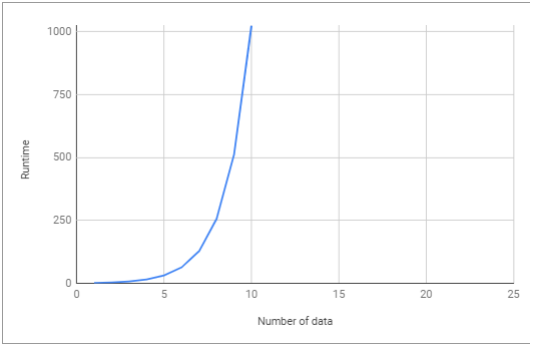
\includegraphics[scale=0.5]{figures/quadric_time}
    \caption{\textit{Quadratic Time}}
    \label{quadrat}
\end{figure}

\item O(2\^n) — Exponential Time
Exponential Time biasanya digunakan dalam situasi dimana kita tidak terlalu tahu terhadap permasalahan yang dihadapi, sehingga mengharuskan kita mencoba setiap kombinasi dan permutasi dari semua kemungkinan.
\begin{figure}[H]
    \centering
    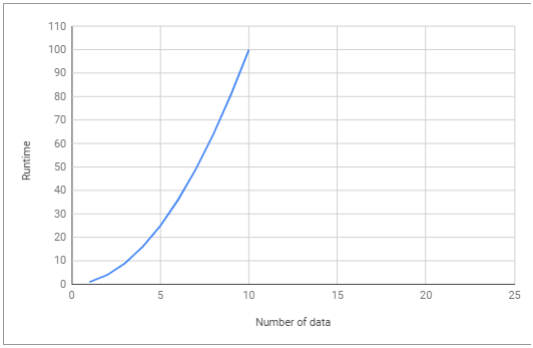
\includegraphics[scale=0.5]{figures/exponential_time}
    \caption{\textit{Exponential Time}}
    \label{exponential}
\end{figure}
\end{enumerate}